\documentclass[12pt, lelterpaper, reqno]{article}\usepackage[]{graphicx}\usepackage[]{color}
%% maxwidth is the original width if it is less than linewidth
%% otherwise use linewidth (to make sure the graphics do not exceed the margin)
\makeatletter
\def\maxwidth{ %
  \ifdim\Gin@nat@width>\linewidth
    \linewidth
  \else
    \Gin@nat@width
  \fi
}
\makeatother

\definecolor{fgcolor}{rgb}{0.345, 0.345, 0.345}
\newcommand{\hlnum}[1]{\textcolor[rgb]{0.686,0.059,0.569}{#1}}%
\newcommand{\hlstr}[1]{\textcolor[rgb]{0.192,0.494,0.8}{#1}}%
\newcommand{\hlcom}[1]{\textcolor[rgb]{0.678,0.584,0.686}{\textit{#1}}}%
\newcommand{\hlopt}[1]{\textcolor[rgb]{0,0,0}{#1}}%
\newcommand{\hlstd}[1]{\textcolor[rgb]{0.345,0.345,0.345}{#1}}%
\newcommand{\hlkwa}[1]{\textcolor[rgb]{0.161,0.373,0.58}{\textbf{#1}}}%
\newcommand{\hlkwb}[1]{\textcolor[rgb]{0.69,0.353,0.396}{#1}}%
\newcommand{\hlkwc}[1]{\textcolor[rgb]{0.333,0.667,0.333}{#1}}%
\newcommand{\hlkwd}[1]{\textcolor[rgb]{0.737,0.353,0.396}{\textbf{#1}}}%
\let\hlipl\hlkwb

\usepackage{framed}
\makeatletter
\newenvironment{kframe}{%
 \def\at@end@of@kframe{}%
 \ifinner\ifhmode%
  \def\at@end@of@kframe{\end{minipage}}%
  \begin{minipage}{\columnwidth}%
 \fi\fi%
 \def\FrameCommand##1{\hskip\@totalleftmargin \hskip-\fboxsep
 \colorbox{shadecolor}{##1}\hskip-\fboxsep
     % There is no \\@totalrightmargin, so:
     \hskip-\linewidth \hskip-\@totalleftmargin \hskip\columnwidth}%
 \MakeFramed {\advance\hsize-\width
   \@totalleftmargin\z@ \linewidth\hsize
   \@setminipage}}%
 {\par\unskip\endMakeFramed%
 \at@end@of@kframe}
\makeatother

\definecolor{shadecolor}{rgb}{.97, .97, .97}
\definecolor{messagecolor}{rgb}{0, 0, 0}
\definecolor{warningcolor}{rgb}{1, 0, 1}
\definecolor{errorcolor}{rgb}{1, 0, 0}
\newenvironment{knitrout}{}{} % an empty environment to be redefined in TeX

\usepackage{alltt}
\usepackage{setspace, graphicx, fullpage, amssymb, amsmath, epsfig, array, natbib, multirow, hyperref, epstopdf}
\usepackage[T1]{fontenc}
\usepackage{baskervald}
\usepackage{amsfonts, bm}
\usepackage{dcolumn}
\usepackage{subfigure, float}
\usepackage[margin=1in]{geometry}
\usepackage{verbatim}
\usepackage{url}
\usepackage{listings}
\usepackage{tcolorbox}
\usepackage{booktabs}
\usepackage{fancyhdr}
\newcolumntype{d}[1]{D{.}{.}{#1}}

\title{\textbf{Is Democracy Good for the Poor?\\ A Replication Paper}}
\author{Jianzi He\\ he.1009@osu.edu}
\IfFileExists{upquote.sty}{\usepackage{upquote}}{}
\begin{document}

\begin{titlepage}
\maketitle

\doublespacing
\
\
\begin{abstract}
Conventional wisdom holds that democracy improves the welfare of the poor. But Michael Ross challenges this conviction in his 2006 paper published in \textit{American Journal of Political Science}. Ross argues that the previous studies of democracy and the poor suffer from selective bias and failure in controlling the country-specific fixed effect and global trend. When those methodological flaws are corrected, there is no strong evidence for the improvement of the the infant and child mortality as the outcome of democracy. Based on this finding, Ross further argues that democracies may actually more concern about the middle- and upper-income groups than the poor. In this project, I will replicate the main findings of this paper, examine Ross's analysis from causal inference perspective, and discuss potential improvement.
\end{abstract}

\end{titlepage}


\section{Data and Measurements}
Ross's (\citeyear{ross2006democracy}) paper focuses on the causal relation between regime types and infant or child mortality, which is based on a cross-naional five-year panel dataset covering 168 states during the period 1970-2000. This study focuses on two depedent variables: the log of the infant mortality and the log of the child mortality. The independent variable, regime type, is meansured in two different ways: (1) creating a 21-point scale \textit{POLITY} score on the basis of the widely-used Polity IV dataset and (2) using a natural log of cumulative years of being democracy since the year 1900. The latter strategy aims to capture the experience of being democracy, which matters when we compare the performances of democracies between the ``new'' and ``old''. In addition, Ross includes four control variables---the log of income per capita, population density, economic growth, and HIV prevalence rate---and one dummy variable that controls the exogenous global trend for each country-period. Table 1 shows the descriptive statistics of these variables in Ross's dataset(except for the country-period dummy variable).

% latex table generated in R 3.3.1 by xtable 1.8-2 package
% Sun Sep 18 15:35:30 2016
\begin{table}[H]
	\centering
	\caption{Descriptive Statistics}
	\begin{tabular}{lllllllll}
		\hline
		& n & mean & sd & median & min & max & range & se \\
		\hline
		Independent Variables &&&&&&&&\\
		\hline
		Child Mortality(log) & 938.00 & 4.10 & 1.14 & 4.31 & 1.39 & 5.99 & 4.61 & 0.04 \\
		Infant Mortality(log) & 938.00 & 3.80 & 1.02 & 4.03 & 1.10 & 5.42 & 4.32 & 0.03 \\
		\hline
		Dependent Variables &&&&&&&&\\
		\hline
		Polity & 1129.00 & -0.63 & 7.30 & -3.80 & -10.00 & 10.00 & 20.00 & 0.22 \\
		Democracy Years(log) & 1008.00 & 1.44 & 1.69 & 0.00 & 0.00 & 4.62 & 4.62 & 0.05 \\
		\hline
		Control Variables &&&&&&&&\\
		\hline
		GDP per capita(log) & 783.00 & 8.23 & 1.05 & 8.24 & 5.72 & 10.73 & 5.01 & 0.04 \\
		Population Density(log) & 906.00 & 3.66 & 1.51 & 3.69 & -0.16 & 8.73 & 8.89 & 0.05 \\
		GDP Growth(log) & 851.00 & 3.22 & 4.91 & 3.46 & -42.45 & 35.59 & 78.04 & 0.17 \\
		HIV Prevalence Rate(log) & 999.00 & 0.21 & 0.51 & 0.00 & 0.00 & 3.30 & 3.30 & 0.02 \\
		\hline
	\end{tabular}
\end{table}

\section{Causal Relation}
Before replicating Ross's analysis, I use the causal graph recommended by Morgan and Winship (\citeyear{morgan2014counterfactuals}) to examine its causal logic (see Figure 1 below). The independent variable, democracy, has multiple pathes towards infant or child mortality. First, democracy may lead to the change in redistributive policy that benefits the poor by rising their living standard. As a result, the infant and child mortality would decrease. Second, democracy could bring the sustain economic growth, which further improves people's living standard and health facilities on avarage. Finally, a democratic government may also invest more on health facilities as the result of its accountability to constituents.

However, democracy alone cannot account for all the improvement (or deterioration) in infant and child mortalities. The global health trend, international aid, epistemic diseases, and war and conflicts complicate the causal relation. Moreover, some of them create back-door pathes with respect to our causal inference. For example, international aids, which seem to be associated with the regime type, may have the direct effects on economy, living standard, and health facilities, depending on their goals. War and conflicts, too, may confound the causal inference by its association with the regime type, since many studies suggest that democracy is more amicable both inside and outside.

\begin{figure}[H]
	\centering
	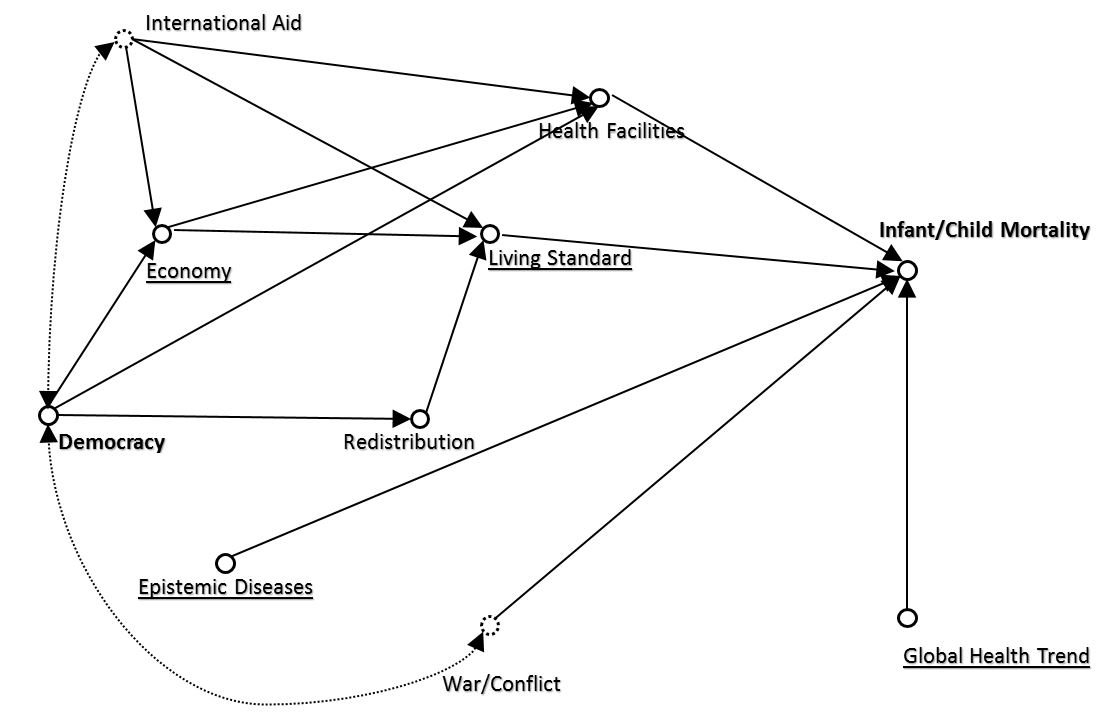
\includegraphics[width=140mm]{cg.jpg}
	\caption{Causal Graph}
\end{figure}

To improve causal inference, Ross chose to control income, population density, economy growth, influencial diseases (HIV as the proxy), and the global health trend. In the causal graph, I underline the corresponding nodes. It is not difficult to see that Ross's strategy is not flawless. Two important nodes---international aid and war/conflict---are completely left out. In addition, the complex relation among democracy, economy, living standard makes two problematic colliders, economy and living standard, and both of them are controlled in Ross's models. Thus, Ross's causal estimation is doomed to be biased to a certain degree.

\section{Methodology and Replication}
Ross estimates the causal effect of democracy on infant/child mortality with two different methods: a fixed-effect model and OLS with panel-corrected standard errors. While the original study was done in STATA, I will try to replicatie his results in R, with the help of ``plm( )'' package for fixed effect models and ``pcse( )'' package for panel-corrected standard errors.

\section*{Appendix: R code}
\begin{tcolorbox}
\begin{knitrout}
\definecolor{shadecolor}{rgb}{0.969, 0.969, 0.969}\color{fgcolor}\begin{kframe}
\begin{alltt}
\hlkwd{library}\hlstd{(causalA16)}
\hlkwd{library}\hlstd{(data.table)}
\hlkwd{library}\hlstd{(ggplot2)}
\hlkwd{library}\hlstd{(texreg)}
\hlkwd{library}\hlstd{(xtable)}

\hlstd{data1} \hlkwb{<-} \hlkwd{load_dataset}\hlstd{(}\hlstr{"Ross_full"}\hlstd{)}
\hlstd{data2} \hlkwb{<-} \hlkwd{load_dataset}\hlstd{(}\hlstr{"Ross_5_year"}\hlstd{)}

\hlcom{# pick up relevant variables and do decriptive statistics}
\hlkwd{attach}\hlstd{(data2)}

\hlstd{x} \hlkwb{<-} \hlkwd{data.frame}\hlstd{(logCMRunicef,logIMRunicef,Polity_1,logDEMYRS_1,}
                \hlopt{+}\hlstd{logGDPcap_1,logDen_1,GDPgrowth_1,logHIV_1)}

\hlkwd{xtable}\hlstd{(}\hlkwd{describe}\hlstd{(x))}
\end{alltt}
\end{kframe}
\end{knitrout}

\end{tcolorbox}

\bibliographystyle{plainnat}
\bibliography{References}

\end{document}
